\subsection{Administrators}

\begin{figure}[!htb]
  \centering
  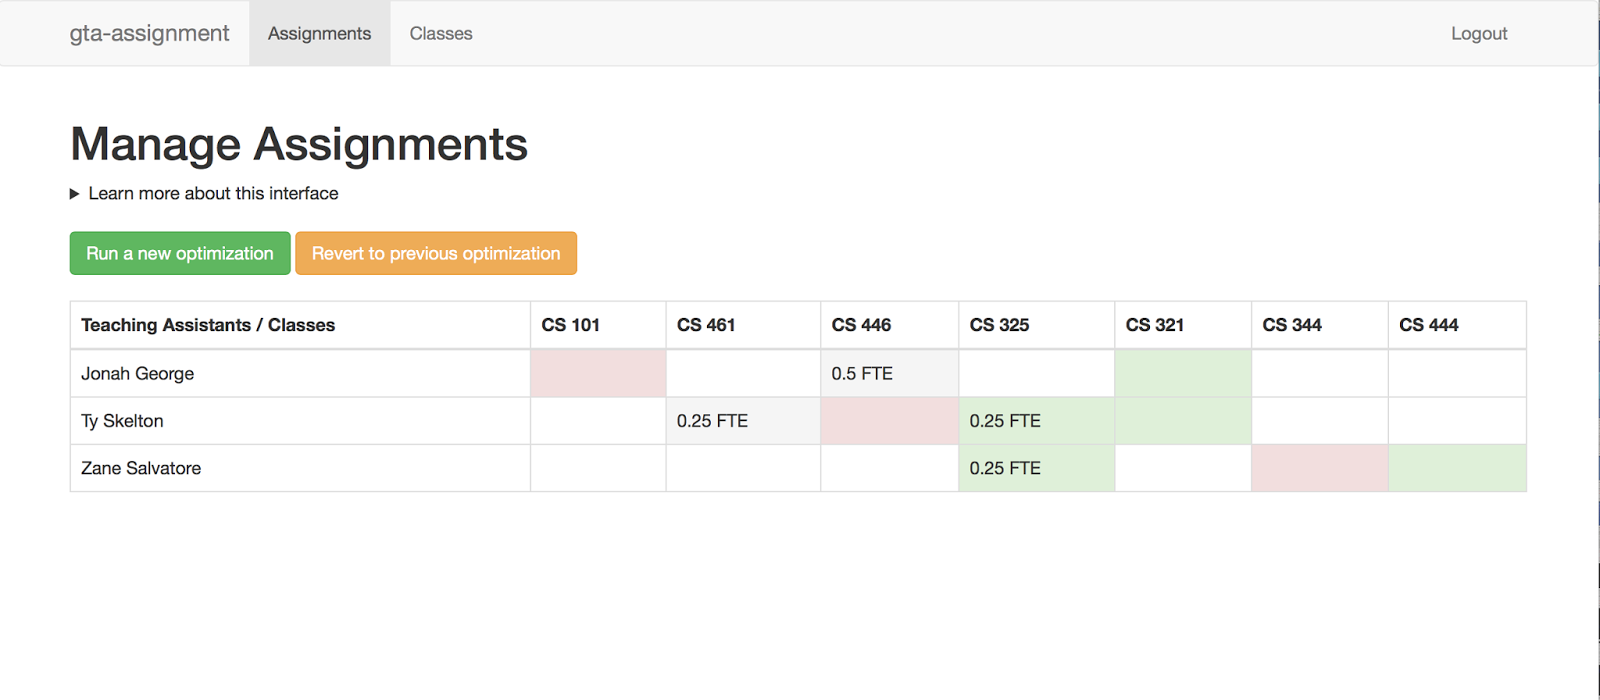
\includegraphics[width=0.75\linewidth]{images/administrator-assignment-design.png}
  \caption{Mock Admin Assignment Page}
\end{figure}

\begin{figure}[!htb]
  \centering
  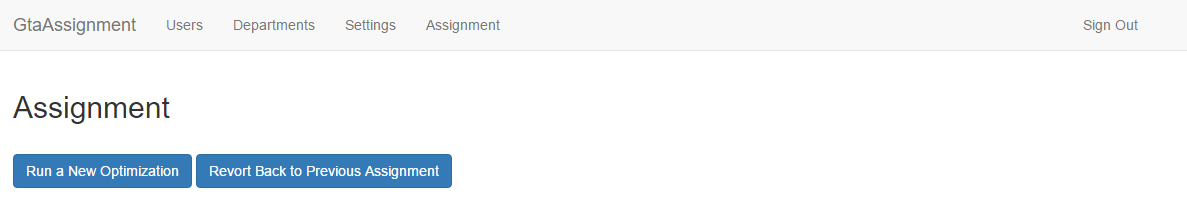
\includegraphics[width=0.75\linewidth]{images/administrator-assignment-alpha.png}
  \caption{Alpha Admin Assignment Page}
\end{figure}

\begin{figure}[!htb]
  \centering
  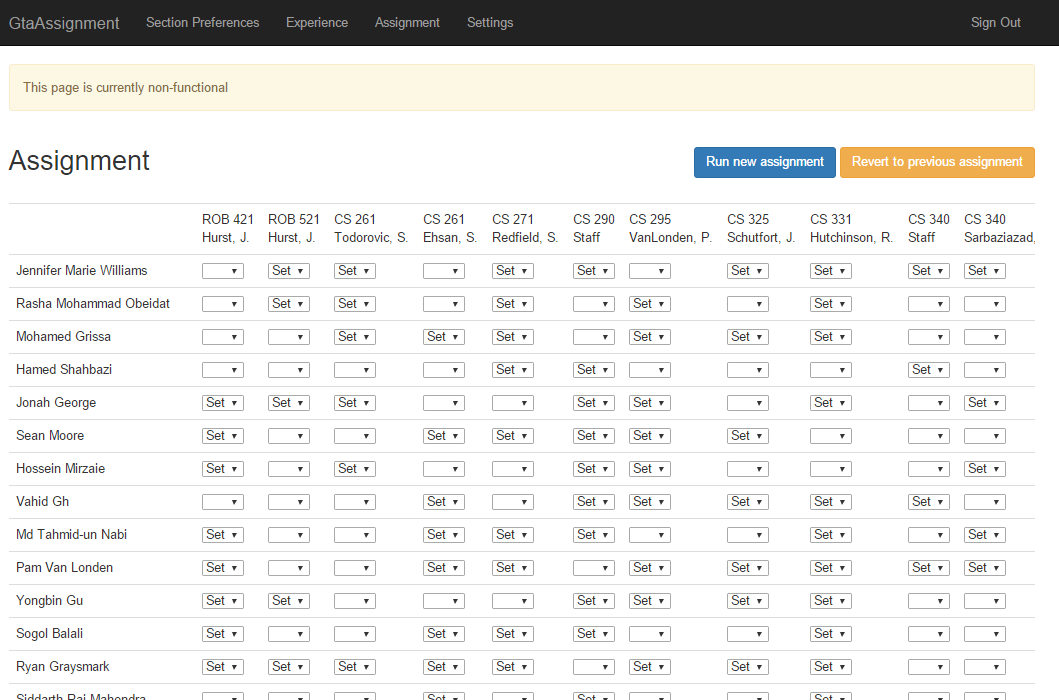
\includegraphics[width=0.75\linewidth]{images/administrator-assignment-beta.png}
  \caption{Beta Admin Assignment Page}
\end{figure}

\begin{figure}[!htb]
  \centering
  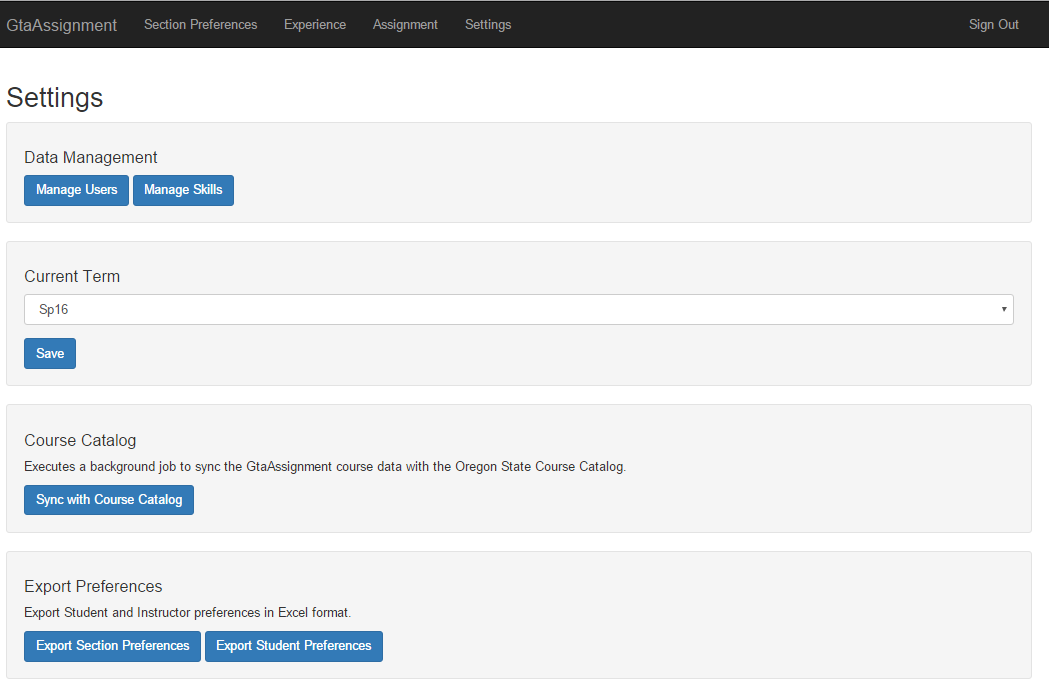
\includegraphics[width=0.75\linewidth]{images/administrator-settings-beta.png}
  \caption{Release Admin Settings Page}
\end{figure}

% \begin{figure}[!htb]
%   \centering
%   \minipage{0.5\textwidth}
%     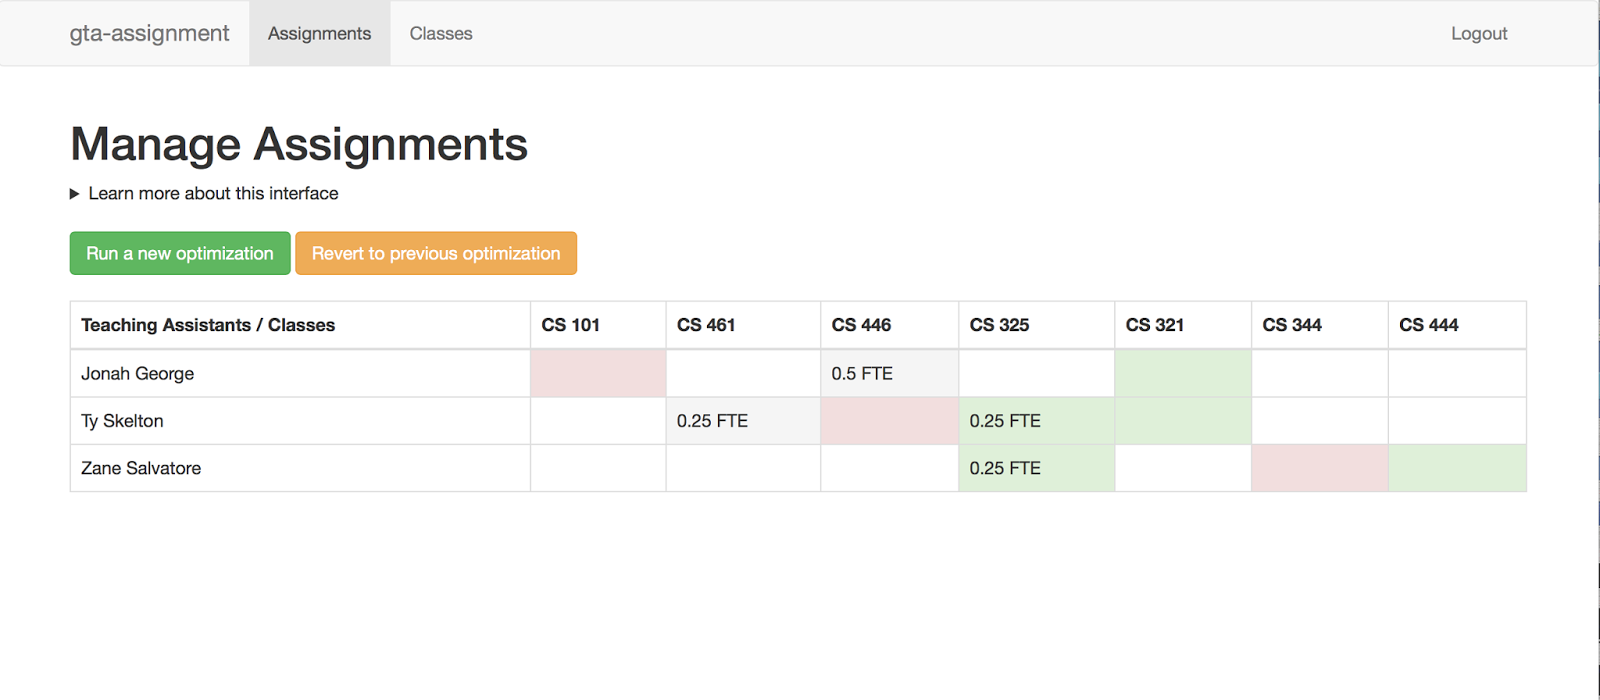
\includegraphics[width=\linewidth]{images/administrator-assignment-design.png}
%     \caption{Mock Admin Assignment Page}
%   \endminipage\hfill
%   \minipage{0.5\textwidth}
%     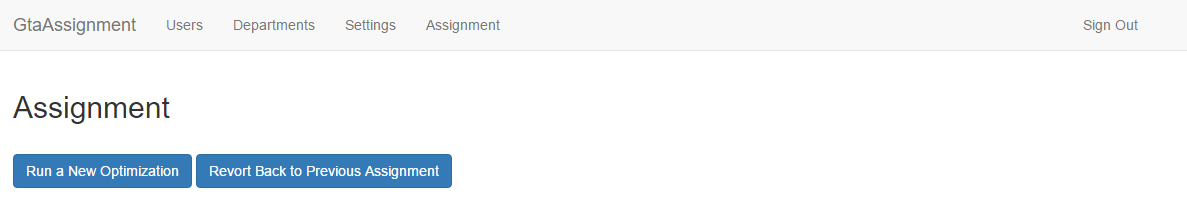
\includegraphics[width=\linewidth]{images/administrator-assignment-alpha.png}
%     \caption{Alpha Admin Assignment Page}
%   \endminipage\hfill
%   \minipage{0.5\textwidth}
%     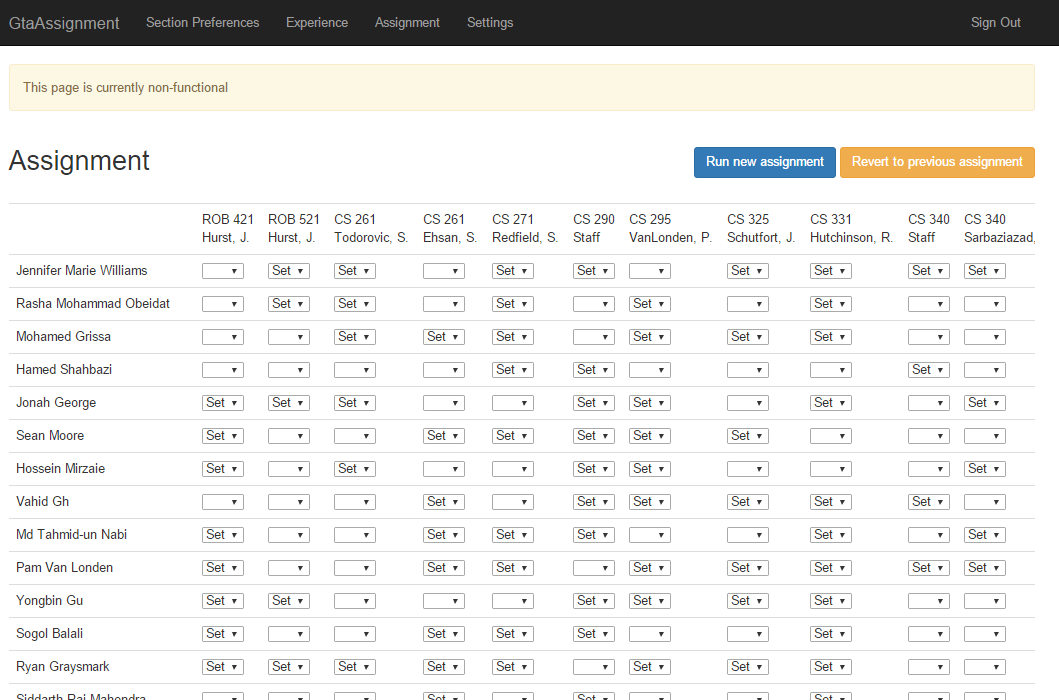
\includegraphics[width=\linewidth]{images/administrator-assignment-beta.png}
%     \caption{Beta Admin Assignment Page}
%   \endminipage\hfill
%   \minipage{0.5\textwidth}
%   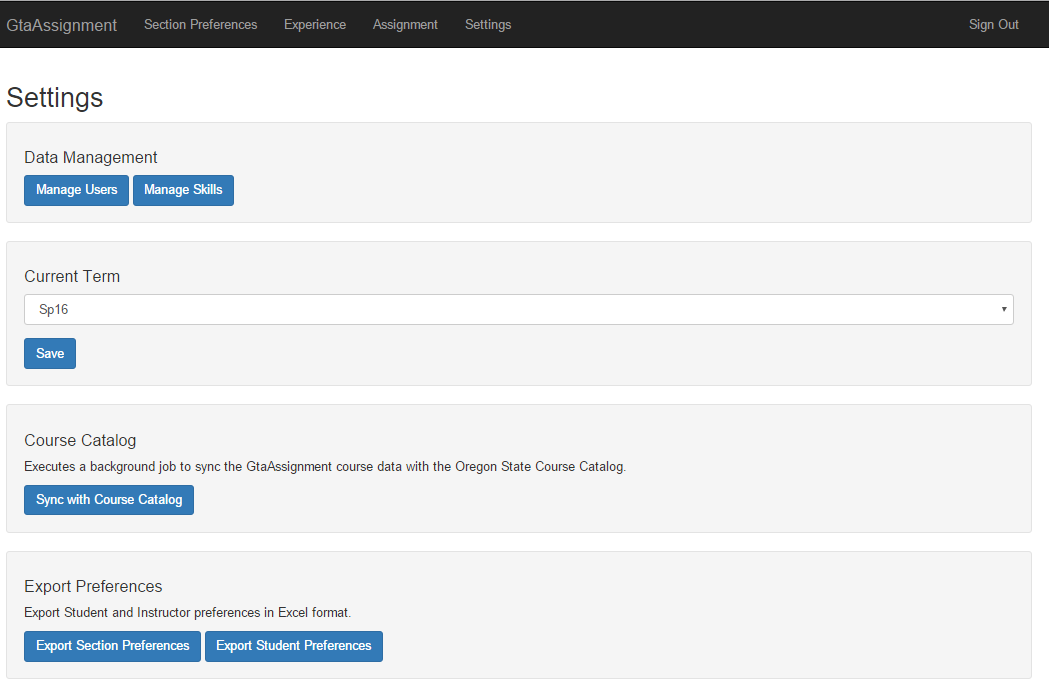
\includegraphics[width=\linewidth]{images/administrator-settings-beta.png}
%   \caption{Release Admin Settings Page}
%   \endminipage\hfill
% \end{figure}

The administrator pages is where most of the action happens.
The administrators have the power to hard code certain students to classes, export both student and instructors preferences.
Administrators also have access to advanced features like manual user and skill management and the ability to re-sync the site with the OSU Course Catalog.
Administrators are an integral part in the whole process- their prior knowledge from assigning TAs to courses will be key in making sure everyone is happy with the results after the ILP has done the heavy-lifting.

Like we pointed out above, the manage users feature has been moved from their the administrators can still modify users like changing their full-time equivalence (FTE) or promoting users to administrator status.
The Current Term field allows the administrators to select the current term which scopes the sections shown throughout the entire site.
The Course Catalog Sync button will trigger a background job update this system's data straight from the OSU Course Catalog.
Finally, the administrators can export the student and instructor preferences to Excel format to be used for reconciling assignment if needed.

\begin{figure}[!htb]
  \centering
  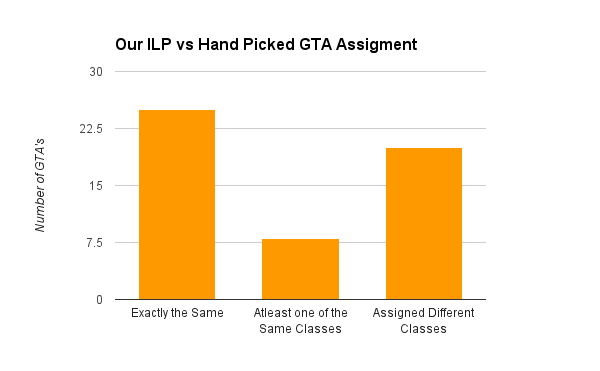
\includegraphics[width=0.75\linewidth]{images/ILPResults.png}
  \centering
  \caption{Our ILP Results vs Hand Picked Results for Winter 2016}\label{ILPresults}
\end{figure}

Using data from the Winter 2016 batch of graduate teaching assistants, we were able to compare the hand picked solution with our LP solution.
A good comparison graph can be seen in figure \ref{ILPresults}.
Our LP was able to assign the exact same class 47.2\% percent of time while also assigning the same class plus another class 15.1\%.
When our algorithm selected different classes, it usually selected students first or second choice 60\% of the time, meaning it was a matter of judgment on the part of those hand picking.
While 37.7\% different assignment might seem high, it is a good result given that there are real world constraints that our system may not capture, e.g. social factors and funding sources.
